\chapter{ روش پیشنهادی }
\section{مقدمه}

همان‌طور که در فصل‌ گذشته شرح داده شد، شناسایی چهره در محیط بدون محدودیت به صورت بی‌درنگ و با دقت بالا با چالش‌های بسیاری همراه است. همچنین دقت بالا و زمان پردازش پایین باهم در تضاد هستند. علاوه بر این‌ها، فرض ‌کمبود داده آموزشی نیز چالش بزرگی محسوب می‌شود. بنابراین در این فصل تلاش می‌کنیم تا روشی برای تشخیص بهتر و دقیق‌تر چهره توسط شبکه عصبی عمیق در تصاویر رنگی پیشنهاد دهیم. و مسئله کمبود داده‌های آموزشی را توسط معماری خاصی از شبکه های GAN برطرف نماییم.
\noindent
از آن‌جایی که ‌شبکه MobileNet معماری بسیار سبک تری نسبت به معماری های شناخته شده دیگر که در فصل ۲ معرفی شدند، دارد؛ بنابراین استخراج ویژگی‌ها از چهره و دسته بندی تصاویر چهره با دقت بالا برای این شبکه بسیار سخت و دشوار است. همچنین در مواردی شباهت چهره افراد به یکدیگر ‌کار را از آن‌چه هست سخت‌تر خواهد کرد. بنابراین ما روشی برای استخراج ویژگی از تصاویر چهره پیشنهاد کرده‌ایم که کمک می‌کند ویژگی‌های استخراج شده که متعلق به دو دسته متفاوت هستند، فاصله بیشتری از هم داشته باشند و در مقابل ویژگی های استخراج شده برای دو تصویر از چهره یک فرد یکسان، فاصله کمتری از هم داشته باشند؛ تا از این طریق بتوان به کاهش مشکلات ذکر شده کمک کرد. این روش شامل بخش‌های تولید چهره، یافتن چهره، آموزش شبکه عصبی پیچشی و ‌استخراج ویژگی می‌باشد.
\section{روش پیشنهادی}
دیاگرام
\begin{figure}[h]
\centering
  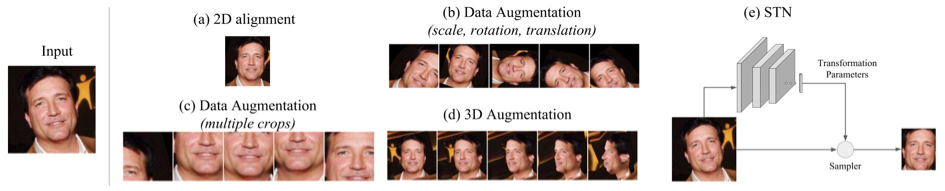
\includegraphics[scale=1]{image3-1}
  \caption{نمای کلی از روش پیشنهادی \cite{ref1}.}
  \label{image2-1}
\end{figure}

\subsection{پیش پردازش}
پیش‌پردازش شامل تصحیح گاما و اعمال فیلتر دوطرفه به منظور حذف نویز پس‌زمینه است. در ادامه به شرح مراحل پیش‌پردازش می‌پردازیم.
\subsubsection{یافتن چهره}
استفاده از رتینا
\subsubsection{تولید تصاویر آموزشی با \lr{GAN}}

در ادامه روند پیش‌پردازش، نوبت به تصحیح گاما می‌رسد. با این هدف که با استفاده از یک تبدیل غیرخطی روشنایی تصویر بهبود یابد. پس از پیش‌پردازش بالا، تصویر نسبت به قبل بهبود پیدا می‌کند اما پس از تکه تکه کردن تصویر جهت آموزش شبکه، تاریک بودن تصاویر مشهود است. برای حل این مشکل از گاما 0.8 استفاده می‌کنیم تا تصویر کمی روشن تر شود.
همچنین با تکه تکه کردن تصویر، نویزهایی در پس‌زمینه مشاهده می‌شود که ممکن است در فرآیند آموزش شبکه را دچار خطا کند. برای حذف این نویزها و در عین حال حفظ لبه‌ها در تصویر از فیلتر دوطرفه  استفاده می‌کنیم.
نتیجه اعمال این دو فرآیند را در تصویر زیر مشاهده می‌کنید. این نکته حائز اهمیت است که نتیجه حدف نویز در تکه‌های ایجاد شده از هر تصویر قابل مشاهده است.

استفاده از اف اس گن
\subsection{آموزش شبکه جهت استخراج ویژگی}
که پیش‌تر بیان شد به آموزش این شبکه می‌پردازیم. مشابه مرحله قبل از شبکه ResNet-50 برای آموزش استفاده می‌کنیم و ساختار آن مشابه آن چیزی است که در شکل ‏3 6 مشاهده می‌کنید. مجموعه داده خود را پس از پیش‌پردازش و افزایش‌ داده‌ها، آماده می‌کنیم. تعداد کل داده‌های آموزش برای این مرحله را به حدود 320000 رساندیم و آموزش را در 30 دوره انجام داده‌ایم.
\subsection{تابع ضرر}
یکی از چالش های اصلی در یادگیری ویژگی ها با استفاده از شبکه های عصبی عمیق پیوسته \lr{(DCNN)} برای شناسایی چهره در مقیاس بزرگ، طراحی تابع ضرر مناسب است که قدرت تفکیک را افزایش می‌دهد. هدف ما کم کردن فاصله بین ویژگی‌های عمیق و مراکز کلاس‌های آن‌ها در فضای اقلیدسی برای دستیابی به فشردگی درون کلاسی بیشتر می‌باشد. ما یک تابع ضرر برای افزایش زاویه ای حاشیه برای دستیابی به ویژگی های بسیار متمایز برای تشخیص چهره پیشنهاد می‌کنیم که عملکرد بهتر برخوردار است و می توان آن را به راحتی با هزینه های محاسباتی ناچیز پیاده سازی کرد.
\noindent
برای آموزش شبکه های عصبی عمیق پیوسته برای تشخیص چهره، دو رویکرد اصلی وجود دارد. روش اول دسته بندی را آموزش می دهند که می تواند هویت های مختلف را در مجموعه آموزش از هم جدا کند، مانند با استفاده از طبقه بندی \lr{softmax}، و رویکرد دوم که مستقیماً یک تعبیه را یاد می گیرند، مانند \lr{triplet loss}. بر اساس داده های آموزش در مقیاس بزرگ و معماری \lr{DCNN}، هر دو روش می توانند عملکرد بسیار خوبی در تشخیص چهره داشته باشند. با این حال، هم رویکرد \lr{softmax} و هم رویکرد \lr{triplet loss} اشکالاتی دارد.
\noindent
برای :
\begin{enumerate}
\item
	اندازه ماتریس تبدیل W به طور خطی با افزایش تعداد دسته ها \lr{(n)} افزایش می یابد.‌
\item 
ویژگیهای آموخته شده برای مسئله‌های طبقه بندی با مجموعه بسته قابل تفکیک هستند اما به اندازه کافی برای مسئله تشخیص چهره که یک مسئله باز می‌باشد، مناسب نیستند. 
\end{enumerate}
\noindent
برای \lr{triplet loss}:
\begin{enumerate}
\item
 برای مجموعه داده های مقیاس بزرگ، رشد شدید در تعداد ترکیب‌های تعداد تصاویر سه گانه وجود دارد که منجر به افزایش قابل توجه تعداد مراحل تکرار می‌شود.
\item 
 استخراج مجموعه تصاویر سه گانه یک مسئله دشوار برای آموزش موثر می‌باشد. 
\end{enumerate}
\noindent
ما برای افزایش بیشتر قدرت تمایز مدل تشخیص چهره و ایجاد ثبات در روند آموزش، تابع ضرر مبتنی بر توابع مثلثاتی را پیشنهاد می‌کنیم. همانطور که در شکل 2 نشان داده شده است، حاصل ضرب نقطه ای مقادیر موجود در ویژگی های استخراج شده و آخرین لایه کاملاً متصل، برابر با ضرب کسینوسی آن‌ها پس از نرمال سازی می باشد‌، ما از تابع مثلثاتی کسینوسی برای محاسبه زاویه بین ویژگی فعلی و وزن هدف استفاده می‌کنیم. سپس یک حاشیه زاویه ای به زاویه هدف اضافه می‌کنیم‌، در انتها با استفاده از تابع کسینوس دوباره مقادیر را به فضای خطی برمی‌گردانیم. مراحل بعدی دقیقاً مانند \lr{softmax} هستند.
مزایای این روش پیشنهادی را می‌توان به شرح زیر خلاصه کرد:
\begin{itemize}
 \item
در مجموعه داده های تصویر و فیلم در مقیاس بزرگ ، به عملکرد مناسبی دست می یابد.
 \item
فقط به چندین خط کد نیاز دارد و اجرای آن در چارچوب های یادگیری عمیق مبتنی بر \lr{Pytorch} و \lr{Tensorflow} آسان است. برای داشتن عملکرد پایدار نیازی به ترکیب با سایر توابع ضرر ندارد و به راحتی همگرا می‌شود.
 \item
هنگام آموزش فقط پیچیدگی محاسباتی ناچیز را اضافه می کند. پردازنده های گرافیکی کنونی می توانند به راحتی از هزاران دسته مختلف برای آموزش پشتیبانی کنند و مدل به راحتی می تواند هویت های بیشتری را پشتیبانی کند.
\end{itemize} 
\noindent


رابطه ریاضی \lr{softmax} معروف ترین تابع ضرر طبقه بندی که به طور گسترده استفاده می شود، به شرح زیر است:
 \begin{equation}\label{eq3-2}
L= - \frac{1}{N} \sum_{i=1}^{N} log \frac{e^{{W_{y_i}^T} x_i + b_{y_i}}}{\sum_{j=1}^{n} e^{{W_j^T} x_i + b_j}} 
\end{equation}
\noindent
که در آن \lr{xi} نشان دهنده ویژگی عمیق نمونه \lr{i} ازدسته \lr{y} است. تعداد ابعاد ویژگی استخراج شده را 512 در نظر گرفتیم. \lr{Wj} ستون \lr{j}  ام از وزن \lr{W} می‌باشد و \lr{bj} بایاس است. مقدار \lr{N}اندازه دسته و \lr{n} تعداد دسته‌ها است. این تابع مستقیما ویژگی استخراج شده را برای اعمال شباهت بالاتر برای نمونه های درون کلاس و فاصله بیشتر برای نمونه های بین کلاسی بهینه نمی‌کند، که منجر به ایجاد مشکل در عملکرد آن برای تشخیص چهره عمیق تحت تغییرات ظاهری بزرگ درون کلاس می شود (به عنوان مثال تغییرات زاویه چهره و تقییرات سنی).

\noindent
ما رابطه فوق را مبنای محاسبات قرار دادیم و تغییرات جزیی به آن اضافه کردیم. برای سادگی مقدار بایاس را صفر در نظر گرفتیم. سپس حاصل ضرب مقادیر موجود در ویژگی های استخراج شده و آخرین لایه کامل
متصل را به صورت
$W_j^T x_i = ||W_j|| ||x_i|| cos(θ_j)$
تبدیل می کنیم، که \lr{θj} زاویه بین وزن \lr{Wj} و ویژگی \lr{xi} است. نرمال سازی ویژگی‌ها و وزن‌ها باعث می‌شود که خروجی فقط به زاویه بین ویژگی و وزن بستگی داشته باشد. به کمک نرمال سازی مقادیر وزن $||W_j||$ را برابر ۱ در نظر می‌گیریم. همچنین ویژگی استخراج شده $||x_i||$ را نرمال کرده و نام آن را \lr{s} در نظر می‌گیریم. ‌‌‌بنابرین ویژگی‌های استخراج شده در یک ابر کره با شعاع s توزیع می‌شوند. برای افزایش حاشیه بین \lr{xi} و \lr{Wj} یک مقدار \lr{m}اضافه می‌کنیم تا به طور همزمان فشرده سازی درون کلاسی و اختلاف بین کلاسی را افزایش دهیم.
 \begin{equation}\label{eq3-2}
L = - \frac{1}{N} \sum_{i=1}^{N} log \frac{e^{s(cos(\theta_{y_i}+m))}}{e^{s(cos(\theta_{y_i}+m))} + \sum_{j=1}^{n} e^{s(cos(\theta_j))}}
\end{equation}
\noindent
همانطور که در شکل 3 نشان داده شده است، \lr{softmax} ویژگی‌های تقریباً قابل تفکیکی ایجاد می‌کند اما در مرزهای تصمیم گیری ابهام قابل توجهی به وجود می‌آید، در حالی که تابع ضرر ما می تواند فاصله بیشتری را بین دسته‌های نزدیک اعمال کند.
\begin{figure}[h]
\centering
  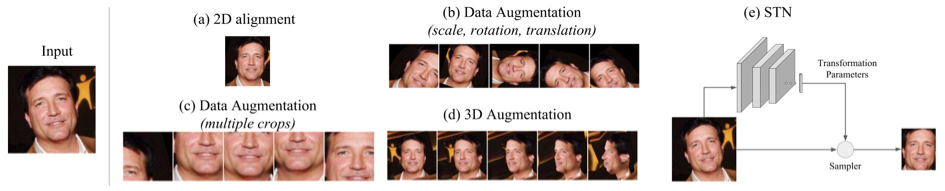
\includegraphics[scale=1]{image3-1}
  \caption{رویکردهای مختلف هم ترازی چهره \cite{ref1}.}
  \label{image2-1}
\end{figure}

\subsubsection{مدل پيشنهادي پايه}
حال نوبت آن است که معماری مناسب شبکه برای مسئله را به دست آوریم. با آزمایش‌های مختلف بر روی شبکه‌های به‌روز و متداول از جمله
\lr{MobileNet},
\lr{MobileNetV2},
\lr{NASNetMobile},
\lr{VGG19}،
\lr{ResNet-50}،
\lr{EfficientNetB0},
و
\lr{IncetionResNetV2}
به کمک یادگیری انتقال انجام دادیم. آزمون را بر روی حدود 20000 تصویر چهره ارزیابی بر روی مجموعه داده های زیر‌ انجام داده‌ایم. نتایج سه شبکه برتر از نظر معیار‌ ارزیابی دقت در جدول ‏3 3 مشاهده می‌کنید. 
\begin{center}
\begin{tabular}{|c c c c c|}
\hline 
مقاله ها & چالش مورد نظر & رویکرد & مزیت ها & مشکل ها
\\
\hline 
 [23-26] & حالت چهره	 & تبدیل دوبعدی & 	پیچیدگی محاسباتی قابل قبول & 	استخراج نقاط ویژه باید دقیق تر باشد
 \\
\hline
[22, 27-30] & حالت چهره & 	استفاده از شبکه عصبی عمیق & دقت بالا در شرایط کنترل نشده & 	پیچیدگی محاسباتی، وابستگی به داده های آموزش 
\\
\hline
[11, 31-34] & حالت چهره & 	تبدیل مدل دو بعدی به سه بعدی & 	دقت بالا 	پیچیدگی محاسباتی
\\
\hline
\end{tabular}
\end{center}

آزمایش‌هایی بر روی معماری های مطرح دیگر نیز انجام شد که به علت ضعیف بودن نتایج یا بالا بودن زمان پاسخ دهی در جدول‌ درج نشده‌اند. از نتایج جدول‌ در می یابیم که بهترین معماری شبکه برای مسئله ما معماری \lr{MobileNetV2} است.

در این معماری مسير استخراج ويژگي از پنج لايه كانولوشن، چهار لايه خطي و نرمال ساز چهار لايه ديكانولوشن۳ و شش ماژول  تشکیل شده است، كه در ادامه توضيح داده خواهد شد، تصوير ورودي I به بخش استخراج ويژگي داده ميشود و مدل در اين مسير به طور خودكار يك سلسله مراتب ويژگي را از تصاوير ورودي آموزش خواهد ديد و در نهايت اين ويژگيهاي استخراج شده از لايههاي مختلف با يكديگر تركيب شده و به عنوان ورودي تقسيمبند مورد استفاده قرار ميگيرد ]۱۴[ .

لايه كانولوشن
سه لايه كانولوشن همراه با گام دو، اندازه حجم ورودي را با ضريبي از دو كاهش ميدهد. سايز پنجره فيلترها 3 × 3 ميباشد. دليل انتخاب سايز كوچك پنجره فيلترها كاهش پيچيدگي محاسباتي و همچنين عملكرد خوب آنها در استخراج ويژگي ميباشد. چگونگي عملكرد يك لايه كانولوشن از رابطه ۲.۳ بدست
ميآيد.
 \begin{figure}[h]
\centering
  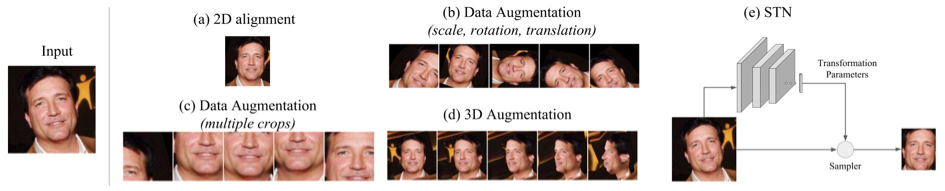
\includegraphics[scale=1]{image3-1}
  \caption{رویکردهای مختلف هم ترازی چهره \cite{ref1}.}
  \label{image2-1}
\end{figure}


\subsubsection{آموزش‌}
در ابتداي روند آموزش، لازم است پارامترهاي مدل مقدار دهي اوليه شوند و انتخاب پارامترهاي اوليه ميتواند تأثير زيادي در مدل آموزش يافته داشته باشد. در اين پژوهش به منظور مقدار دهي اوليه پارامترها از تابع توزيع يكنواخت استفاده شده است. از ديگر چالشهاي اساسي براي روشهاي بهينه سازي مبتني بر گراديان، انتخاب ميزان نرخ يادگيري مناسب است. روشهاي كلاسيك گراديان تصادفي از نرخ يادگيري ثابت يا كاهشي استفاده ميكنند، كه براي همه پارامترهاي مدل يكسان است. با اين حال، مشتقات جزئي پارامترهاي لايههاي مختلف ميتوانند از نظر مقدار متفاوت باشند، كه ميتواند به نرخ يادگيري مختلفي نياز داشته باشد. با اين حال، مشتقات جزئي پارامترهاي لايههاي مختلف ميتوانند از نظر مقدار تفاوت قابل توجهي داشته باشند، كه ميتواند به نرخ يادگيري مختلفي نياز داشته باشد. در سالهاي اخير، تمايل به توسعه روشهايي براي انتخاب خودكار نرخ يادگيري مستقل افزايش يافته است. اكثر روشها )به عنوان مثال، RMSprop، [۴۸]AdaDelta، [۴۷]AdaGrad]۴۹[ و Adam]۵۰[( آمارهاي مختلف مشتقات جزئي را در چندين تكرار جمع آوري ميكنند و از اين اطلاعات براي تعيين ميزان يادگيري سازگار براي هر پارامتر استفاده ميكنند. اين امر به ويژه براي آموزش شبكههاي عميق بسيار مهم است، جايي كه نرخ يادگيري مطلوب اغلب براي هر لايه بسيار متفاوت است. در اين پژوهش در آزمايشات انجام شده از همه روشهاي نام برده استفاده شد ولي روش Adam عملكرد بهتري ارائه داده است.

\subsubsection{دسته‌بندی}
در مرحله آزمون به منظور تشخیص هویت یک تصویر چهره، پس از پیش‌پردازش تصویر را مطابق با ورودی شبکه تغییر اندازه میدهیم و جهت استخراج ویژگی‌ به آن شبکه می‌دهیم. پس از استخراج ویژگی ها توسط شبکه، بردار ۵۱۲ تایی بدست آمده را با بردار های مربوط به چهره های بانک اطلاعاتی مقایسه کرده و با محاسبه فاصله اقلیدسی بردار ها، نزدیک ترین شخص مورد نظر انتخاب شده و در صورتی که فاصله میان بردار ویژگی آن ها از حد آستانه کمتر باشد. عمل دسته بندی انجام شده و هویت چهره مورد نظر تعیین می شود. در غیر این صورت اعلام میداریم که شخص مورد نظر قابل شناسایی نمی باشد.

پس از آموزش شبکه در 30 دوره بر روی داده‌های آموزشی، می‌توان از این شبکه برای استخراج پیکسل‌های کاندید استفاده کرد.
روند کار برای استخراج پیکسل‌های کاندید به این صورت است که ابتدا بر روی تصویر اصلی با یک تعداد گام کوتاه 5 پیکسل شروع به حرکت می‌کنیم و تکه‌های 33 در 33 پیکسل استخراج می‌کنیم. تکه‌های استخراج شده را جهت ارزیابی به شبکه می‌دهیم و احتمال بیمار بودن را به تک تک پیکسل‌های داخل آن تکه تخصیص می‌دهیم.
با این روش به جز پیکسل‌های مرزی، سایر پیکسل‌ها در چندین تکه حضور دارند. بنابراین دو ماتریس به اندازه طول و عرض تصویر فوندوس تشکیل می‌دهیم. یکی از این ماتریس‌ها مشخص می‌کند که هر پیکسل در چند تکه‌ حضور داشته است (Count). و دیگری مجموع احتمالات هر پیکسل که در تکه‌های ارزیابی حضور داشته است را در خود نگهداری می‌کند (SumOfProbs). در نتیجه میانگین احتمال بیمار بودن هر پیکسل از طریق رابطه (3-1) به دست می‌آید.

 
شکل ‏3 8- نمونه‌ای از خطوط برش تقاطعی و نمایه‌های برش تقاطعی از کاندید‌های میکروآنوریسم بازچاپ از [55]. a میکروآنوریسم صحیح و b و c کاندید‌های اشتباه هستند.

	آموزش SVM برای دسته‌بندی کاندیدها
تا این‌جا توانسته‌ایم سه نوع ویژگی را استخراج کنیم. نوع اول، ویژگی‌هایی است که از طریق آموزش شبکه عصبی پیچشی به دست می‌آید. نوع دوم ویژگی‌های مبتنی بر نمایه برش تقاطعی و نوع سوم ویژگی‌های مبتنی تبدیل برش تقاطعی است. حال از تمام ویژگی‌های منتخب مطابق شکل ‏3 10 برای آموزش یک ماشین بردار پشتیبان (SVM) استفاده می‌کنیم و در مرحله آزمون، ویژگی‌های عنوان شده را استخراج کرده و به کمک یک ماشین بردار پشتیبان سالم و یا بیمار (دارای میکروآنوریسم) بودن آن تکه را مشخص می‌کنیم. 
 
شکل ‏3 10- دسته‌بندی ویژگی‌های استخراج شده از تکه به کمک ماشین بردار پشتیبان

\section{فناوری های استفاده شده}
پیاده‌سازی این الگوریتم به کمک زبان برنامه‌ نویسی پایتون و کتابخانه \lr{PyTorch} و \lr{OpenCV}انجام شده است. از کتابخانه‌های مهم مورد استفاده دیگر در این کار می‌‌توان به \lr{NumPy} برای انجام محاسبات ماتریسی و \lr{SciPy} و \lr{Scikit Learn} اشاره کرد.[35] 

برای آموزش شبکه عصبی مربوط به دسته بندی ۱۲ گیگابایت حافظه اصلی و ۱۲ گیگابایت حافظه گرافیکی در اختیار گرفتیم.

